\section{Cached-feature controls and covariance sensitivity}\label{sec:support}
These additional experiments were specified after the original outcomes were available and are descriptive, post hoc, and unadjusted for multiple comparisons. They do not constitute a new independent confirmation and do not select a replacement model. All seven variants and all four covariance scales are reported. Training uses the 132 development families. Their original six folds are reproduced by sorting family identifiers by SHA-256 and assigning consecutive families modulo six; normalization and fitting occur inside each training fold. The 72 previously evaluated families receive models fitted on all development families only. Both cohorts were already available during study design, so the original inference remains primary.

The numerical-only and complete configurations are controls. Pooled-only zeros the 16 normalized position-correction channels; position-only zeros the 32 pooled-state channels. All visual fits retain 48 allocated input dimensions, the same penalty and the same numerical head, although the numbers of nonzero channels differ. These are component controls within the trained observation decoder, not an independent motion tracker or a replacement frozen video encoder. The direct-target variant fits the visual head to the original anchor-standardized target instead of the remaining numerical residual, while retaining numerical addition. The unclipped variant removes both clipping operations during training-target construction and prediction. The no-fallback variant retains the trained generalized-bounce correction. Removing the coordinate mask alone would be uninformative because the fitted heads already have only active-coordinate outputs; no general mask ablation is claimed.

\par\begin{table}[htbp]\centering\small
\caption{Post hoc cached-feature experiments. Action errors are in millimeters. Development uses six-fold family predictions. Previously evaluated data are descriptive; differences and unadjusted paired 95\% intervals are relative to the original full model.}
\label{tab:support_readout}
\begin{tabular}{lrrrr}\toprule Variant & Development & Evaluated & Difference & 95\% interval\\\midrule
Numerical only & 1.371928 & 1.468770 & $+0.01565$ & $[-0.00053,+0.03114]$ \\
Original full & 1.352231 & 1.453122 & reference & -- \\
Pooled states only & 1.367787 & 1.468546 & $+0.01542$ & $[+0.00684,+0.02396]$ \\
Position corrections only & 1.351850 & 1.451762 & $-0.00136$ & $[-0.01359,+0.00976]$ \\
Direct visual target & 1.365456 & 1.475368 & $+0.02225$ & $[-0.00217,+0.04682]$ \\
Unclipped heads & 1.364726 & 1.484064 & $+0.03094$ & $[-0.00026,+0.07912]$ \\
No bounce fallback & 1.401275 & 1.494771 & $+0.04165$ & $[+0.03078,+0.05253]$ \\
\bottomrule\end{tabular}\end{table}\par

The full and numerical predictions reproduce the original saved outputs and scores within an absolute tolerance of $10^{-12}$; their development scores also match the original six-fold records. Pooled-only provides little point improvement over numerical-only, whereas position corrections retain the measured residual signal. Position-only and full have overlapping paired uncertainty. Direct-target and unclipped variants have higher point errors, but their evaluated-cohort differences from full include zero. Removing generalized-bounce fallback worsens mean action error on both cohorts. These controlled configurations provide evidence about this implementation, without establishing universal safety or a semantic-language contribution.

\subsection{Mean-fixed covariance sensitivity}
For each scale $\beta\in\{0,0.05,0.10,0.20\}$, the full model mean is held fixed and $\Sigma_\beta=C+\operatorname{diag}[(\beta d)^2]$. The existing evaluated cohort is rescored without refitting. The original model remains at $\beta=0.10$; this is descriptive sensitivity rather than confirmation-cohort reselection.

\par\begin{table}[htbp]\centering\small
\caption{Post hoc covariance-scale sensitivity with the complete mean fixed. Width is the mean coordinate-projected joint-region diameter relative to Huber; NLL and CRPS use transformed properties.}
\label{tab:support_covariance}
\begin{tabular}{lrrrr}\toprule Scale & NLL/dim. & CRPS & 90\% coverage & Width ratio\\\midrule
0.00 & -2.532473 & 0.01310272 & 0.968056 & 1.000000 \\
0.05 & -2.538692 & 0.01310534 & 0.971759 & 1.000560 \\
0.10 & -2.545938 & 0.01311324 & 0.973611 & 1.002236 \\
0.20 & -2.543325 & 0.01314513 & 0.977315 & 1.008857 \\
\bottomrule\end{tabular}\end{table}\par

The original scale has the lowest NLL of the four values, whereas zero inflation has the lowest CRPS. Coverage increases with inflation and is already conservative at zero inflation. Thus inflation is not uniformly beneficial across scores and is not responsible for the whole proper-score gain over the robust anchor. Action error is identical at every scale. The width calculation uses $2\sqrt{\chi^2_{k,0.9}\Sigma_{jj}}$, averaged over active coordinates and the existing family/protocol units; it measures coordinate projections, not principal eigen-axis lengths.

\begin{figure}[htbp]\centering
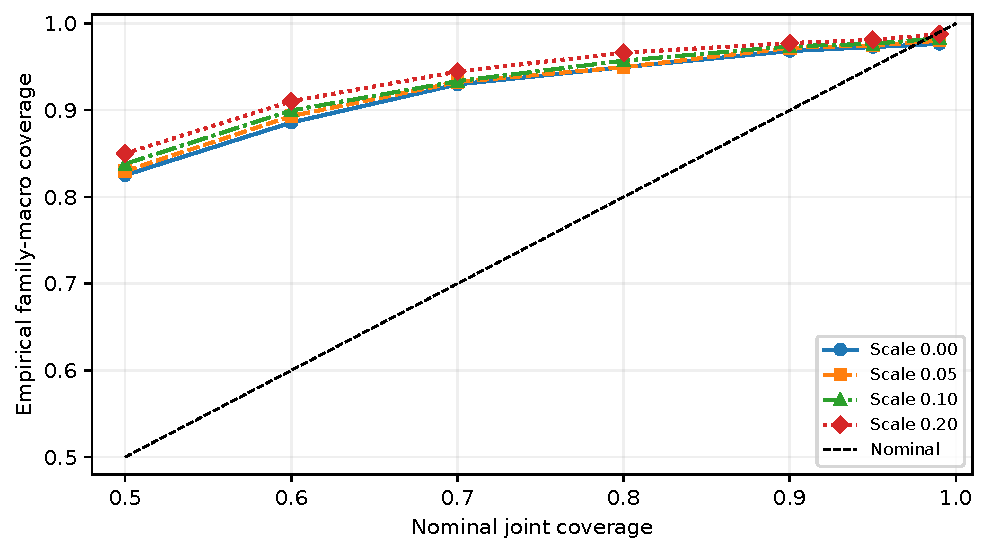
\includegraphics[width=.84\textwidth]{figures/support_coverage.pdf}
\caption{Post hoc empirical coverage at seven nominal levels, recalculated from saved predictions with the complete mean fixed. Symbols and line styles identify covariance scales. The diagonal indicates nominal coverage; no independent calibration sample or confidence bands are introduced.}
\label{fig:support_coverage}
\end{figure}

\subsection{Initialization Jacobian audit}
The input cache contains the physical derivative matrix $J$ and nuisance derivative matrix $J_n$ at the observation initializer. Residuals are divided by observation noise and physical perturbations are measured in prior-standard-deviation units. We reconstruct $J_\perp=J-J_nJ_n^+J$ using the recorded nuisance dimensions and a pseudoinverse cutoff of $10^{-8}$. It exactly matches the stored projected derivative in this cache. These are initialization derivatives, not final robust-anchor derivatives or separate setup-bounce derivatives. Singular values below $\max(10^{-10},10^{-8}s_{\max})$ count as zero.

\par\begin{table}[htbp]\centering\small
\caption{Post hoc singular-value audit of the active initialization subspace. Condition medians use full-rank rows. All entries are in the cache\textquotesingle s standardized coordinate system.}
\label{tab:support_jacobian}
\begin{tabular}{lrrrr}\toprule Protocol & Full rank / rows & Median $s_{\min}$ & 10th pct. $s_{\min}$ & Median condition\\\midrule
multiple forces & 360/360 & 0.6557 & 0.5532 & 11.3110 \\
unforced slide & 360/360 & 3.6974 & 3.4170 & 1.0000 \\
bounce & 360/360 & 21.0018 & 18.9655 & 1.0000 \\
\bottomrule\end{tabular}\end{table}\par

The one-dimensional condition number is identically one for a nonzero column and does not itself indicate strong information. Inactive derivative columns are zero by construction in the initializer; this audit therefore cannot establish that the protocol mask equals the null space of an unrestricted physical model. Initial full rank does not remove nonlinear contact ambiguity or guarantee stable posterior inference. In particular, full rank of the bounce initialization does not invalidate the empirically selected final fallback.
